\section{Introduction}
\label{sec:introduction}

\begin{figure}[t]
 \centering
 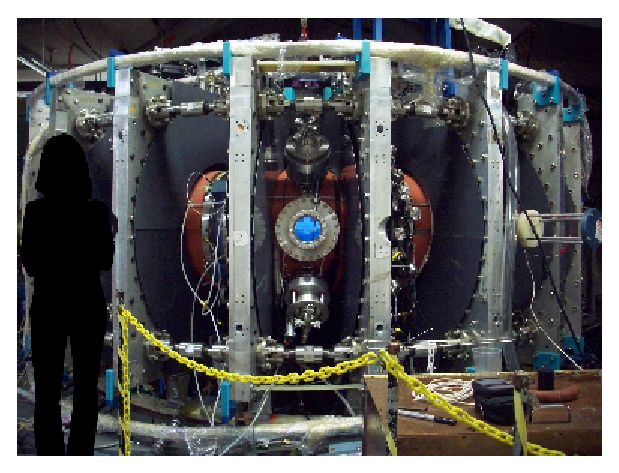
\includegraphics[width=0.82\hsize]{eps/tokamak.eps}
 \caption{Columbia's HBT-EP ``Tokamak''.}
 \label{fig:tokamak}
\end{figure}

Cyber-physical systems (CPS) represent next generation networked and
embedded systems, tightly coupled with computation and physical
elements to control real-world phenomenon.
Their control algorithms, therefore, are becoming more and more complex,
which distinguishes CPS from traditional safety-critical embedded
systems.
Specifically, ``real-fast'' is usually as important as ``real-time''.
This double-edge real-fast and real-time requirement of CPS imposes a
core challenge on systems technology.

Plasma control for fusion is an applications of energy CPS where
complex algorithms must run at a very high rate.
Figure~\ref{fig:tokamak} shows the HBT-EP high-beta ``Tokamak'' device at
Columbia University~\cite{Maurer_PPCF11,Rath_FED12}.
It must process 96 inputs and 64 outputs of data in a few microseconds
to magnetically control the 3-D perturbed equilibrium state of the
plasma~\cite{Boozer_PP99}.
An initial attempt at Columbia University employed fast cutting-edge
CPUs or FPGAs, but even a simplified algorithm failed to meet 20$\mu$s.
An alternative was to parallelize the algorithm using the
graphics processing unit (GPU) and CUDA~\cite{CUDA}, which is the most
successful parallel computing technology.
However, GPU programming is currently not tailored to integrate
sensor and actuator devices.
This is due to the fact that the current GPU programming stack is
completely independent of I/O device drivers.
Since it can take tens of microseconds to transfer hundreds of bytes
data between the CPU and the GPU, the state of the art is not adequate
to apply the GPU for plasma control in real-time.
This is a significant problem for not only plasma control but also any
CPS applications that are augmented with compute devices.

In order to effectively utilize the GPU for low-latency large-data CPS
applications, the system must support a direct communication scheme that
bypasses the data transfer between the CPU and the GPU by connecting the
GPU and I/O devices directly.
To the best of our knowledge, however, there is currently no
standardized support for such a direct data transfer mechanism other than
specialized commercial products for the InfiniBand
network~\cite{GPUDirect}.
To mitigate the data transfer overhead, some programming frameworks
support host memory allocation, letting the GPU directly access data on
the host memory.
This scheme is ill-suited for low-latency GPU computing due to the high
cost of GPU's data access to host memory.
Given that GPU technology is increasingly deployed in
CPS~\cite{Hirabayashi_REACTION12, Mangharam11, McNaughton_ICRA11,
Michel_IROS07}, 
and basic real-time resource management techniques for the GPU are
starting to be developed \cite{Elliott_RTS12, Elliott_ECRTS12, Kato_RTAS11,
Kato_RTSS11, Kato_ATC11, Kato_ATC12, Liu_PACT12}, it is time to look
into tighter integration of I/O processing and GPU computing.

\textbf{Contribution:}
This paper presents a new \emph{zero-copy} I/O processing scheme for GPU
computing.
This scheme allows I/O devices to directly transfer data to and from the
GPU by mapping of memory and I/O address space.
We investigate the problem of existing schemes for low-latency GPU
computing, and demonstrate performance advantages of our zero-copy
scheme with a case study using Columbia's Tokamak device.
Experimental results show the clear benefit of our zero-copy scheme on
the plasma period.
We also provide microbenchmarks to highlight more generic
properties of the I/O processing schemes.
By clarifying these capabilities, we aim to not only improve performance
but also broaden the scope of CPS that can benefit from state-of-the-art
parallel computing technology.

\textbf{Organization:}
The rest of this paper is organized as follows.
Section~\ref{sec:system_model} describes the system model and
assumptions behind this paper.
Section~\ref{sec:io_processing} proposes our zero-copy I/O processing
scheme, and differentiates it from the existing schemes.
Section~\ref{sec:implementation} presents details of system
implementation.
In Section~\ref{sec:case_study}, a case study of plasma control is
provided to demonstrate the real-world impact of our contribution.
Microbenchmarks are also used to evaluate more generic properties of the
I/O processing schemes in Section~\ref{sec:benchmarking}.
Section~\ref{sec:related_work} introduces related work, and this paper
concludes in Section~\ref{sec:conclusion}.